\section{Experiments and Preliminary Results}
\label{sec:experiments}

\subsection{Setup}
All experiments use the Flickr8k training split (halves A and B, 3{,}000 images each) and the 1{,}000-image validation split; the test split has not been read. Visual features are cached once (Section~\ref{sec:design-captioner}). Every GPU stage ran on a single Colab A100: caching BLIP and OWLv2 features for 7{,}000 images took under ten minutes, decoder fine-tuning \FtMinutes{} minutes, and one Retell training run about seven minutes. All scripts and the order in which they were run are in the project repository; the numbers in this section are inserted by the scripts that computed them.

Because human labels do not exist yet, several measurements below compare claims with the five reference captions. A claim whose class no reference mentions is called \emph{reference-unsupported}. This is a proxy, not a correctness judgement, and Section~\ref{sec:exp-check} shows how far it is from one.

\subsection{Current Look/Check Development on B}
The latest update preserves the captioner's attention maps and the frozen OWLv2 checker. On $B_{\mathrm{fit}}$ human boxes, removing the minimum-side filter raises top-three region coverage from \LCRLookBefore\% to \LCRLookAfter\%; for small annotated objects, counting a hit only when it lands on the small box itself, coverage is \LCRSmallBefore\% with the filter and \LCRSmallAfter\% without it. These are B development results, not new validation or test estimates. The selected Check uses the maximum class score across the attended candidates, with image-fold B-fit proxy precision \LCRCheckPrecision{}, wrong-claim recall \LCRCheckRecall{} and informedness \LCRCheckJ{}. Its Look selection had already seen B-fit boxes, so this is conditional Check cross-validation rather than a fully nested estimate of the whole pipeline.

There are \LCRFitImages{} B-fit and \LCRCalImages{} B-cal images. Final score scales and thresholds use only B-cal. Alternative-reference agreement remains limited and does not establish replacement correctness. The new implementation passes evidence-contract and fixed-draft live-replay checks, but the same-detector crop re-encoding experiment and new Retell training have not run. Validation was not reopened for these choices; subsequent results below retain their historical method identities.

\subsection{Drafting Captioner}
\label{sec:exp-captioner}
Table~\ref{tab:caption} compares the public BLIP-base captioning checkpoint with the same model after fine-tuning its decoder on half A for three epochs (AdamW~\cite{loshchilov2019decoupled}, learning rate $2\cdot10^{-5}$, one-cycle schedule, batch 32). Validation CIDEr peaked after the first epoch and slowly declined afterwards while the training loss kept falling (Fig.~\ref{fig:ft}), so the epoch-\FtBestEpoch{} checkpoint is the frozen captioner B0 for everything that follows. Fine-tuning mostly adapts the style of the captions to Flickr8k: drafts contain more claims (\ValClaimsPerImage{} per image instead of 1.84), while the reference-unsupported rate stays roughly where it was (\ZsRUOR\% $\to$ \FtRUOR\%). A better-scoring captioner is therefore not automatically a more faithful one, which is the observation that motivates the project~\cite{rohrbach2018object}.

\begin{table}[t]
\caption{Captioning quality on the Flickr8k validation split (1{,}000 images). Full COCO outputs are unavailable locally; BLEU-4 and CIDEr use the stored alphabetic-tokenisation scores. A dash marks an unavailable metric. 
BLEU-4, METEOR, ROUGE-L, SPICE $\times100$. RUOR: share of generated vocabulary claims that
no reference mentions (reference agreement, \emph{not} a hallucination rate).}
\label{tab:caption}
\centering\footnotesize\setlength{\tabcolsep}{3pt}
\begin{tabular}{@{}lcccccc@{}}
\toprule
Captioner & B-4 & M & R-L & CIDEr & SPICE & RUOR \\
\midrule
BLIP zero-shot & 25.6 & -- & -- & 0.669 & -- & 14.0 \\
BLIP fine-tuned on A (B0) & 32.6 & -- & -- & 0.979 & -- & 15.8 \\
\bottomrule
\end{tabular}
\end{table}


\begin{figure}[t]
\centering
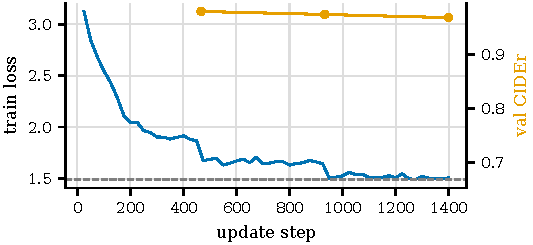
\includegraphics[width=\columnwidth]{figures/finetune_curve.pdf}
\caption{Decoder fine-tuning on half A: training loss (blue) and validation CIDEr after each epoch (orange); dashed: zero-shot CIDEr.}
\label{fig:ft}
\end{figure}

\subsection{Claims and the Limits of the Reference Proxy}
\label{sec:exp-check}
B0 produces \ValClaims{} vocabulary claims on the validation images. Of these, \RefSupportedAll\% are mentioned by at least one reference: \RefSupportedPerson\% of \emph{person} claims, \RefSupportedThing\% of \emph{thing} claims and \RefSupportedStuff\% of \emph{stuff} claims. The remaining claims are not necessarily wrong. For \UnsupThingHighDet\% of the \UnsupThingN{} reference-unsupported \emph{thing} claims, OWLv2 finds the claimed class somewhere in the image with a score above the support threshold. Many of these are plausibly real objects that the five annotators simply did not mention; the pilot labels will show how many. Conversely, the detector's best score for the claimed class separates reference-supported from reference-unsupported claims only moderately: the AUROC is \AurocPerson{} for persons, \AurocThing{} for things and \AurocStuff{} for stuff. Two conclusions follow. First, reference agreement cannot stand in for correctness, which confirms the decision to use human judgement as the primary measure. Second, the detector is markedly weaker on amorphous \emph{stuff} classes, which justifies reporting the three kinds separately.

\subsection{Look: Is Cross-Attention a Usable Localisation Signal?}
\label{sec:exp-look}
We now evaluate against human-drawn Flickr30k Entities boxes, independently of the detector's class predictions. Of \LookAllClaims{} validation claims, \LookGtClaims{} have matching boxes (\LookCoverage\%). Table~\ref{tab:look-human} separates changes to the map from changes to the region rule. The B3 class-conditioned detector and the proposal oracle are references, not alternative sources for the captioner's map.

\textbf{Map and region gains.} With v1 region selection held fixed, subtracting caption-wide attention raises pointing from \LookRawPoint\% to \LookSinkPoint\% and region accuracy to \LookVOneRegion\%. Keeping that sink map fixed, v2 raises region accuracy to \LookVTwoRegion\%; the detector reference reaches \LookDetectorRegion\%, while the candidate-pool oracle reaches \LookOracleRegion\%. The original region-rule grid contained \LookGridCount{} configurations, chosen on B before validation reporting. Corrected energy metrics integrate the actual union of boxes rather than taking the maximum per-box patch coverage. No model or region configuration was changed to obtain this measurement correction.

\begin{table}[t]
\caption{Human-box localisation on validation (\LookGtClaims{} claims). All entries are percentages.
Energy uses the exact union of annotated boxes. Pointing and energy share the map; region accuracy
also depends on the proposal rule.}
\label{tab:look-human}
\centering\footnotesize
\begin{tabular}{@{}lrrr@{}}
\toprule
Map + region rule & Pointing & Energy & Region \\
\midrule
Raw + v1 & 23.9 & 35.8 & 12.9 \\
Sink + v1 & 88.3 & 73.2 & 55.7 \\
Sink + v2 & 88.3 & 73.2 & 75.3 \\
\bottomrule
\end{tabular}
\end{table}

\begin{table}[t]
\caption{Look v2 region accuracy by kind, against any matching human box at IoU $\geq 0.5$.
B3 uses the claimed class score; oracle asks whether any eligible proposal succeeds. Percentages.}
\label{tab:look-kind}
\centering\footnotesize\setlength{\tabcolsep}{4pt}
\begin{tabular}{@{}lrrrr@{}}
\toprule
Kind & Claims & Look v2 & B3 & Oracle \\
\midrule
All & 1{,}795 & 75.3 & 82.7 & 95.3 \\
Person & 761 & 66.4 & 85.9 & 95.5 \\
Thing & 758 & 83.8 & 83.8 & 95.4 \\
Stuff & 276 & 76.4 & 71.0 & 94.2 \\
\bottomrule
\end{tabular}
\end{table}


\textbf{Does the map add information beyond objectness?} Fixed controls on the development half B give \LookBRegion\% region accuracy for v2, \LookBObjectness\% for objectness alone, and \LookBUniform\% for the same v2 rule with a uniform map. On the matched subset with another-class claim, swapping in that claim's map lowers region accuracy from \LookSwapOwn\% to \LookSwapOther\%. These are development diagnostics, not additional held-out comparisons. They support a contribution from the claim-specific map beyond the shared proposal prior.

\textbf{E1: bounded refinement and closure.} The predefined grid evaluated the same three smoothing widths and twelve exponent pairs per kind on B. A kind changed only if its B improvement reached one point. This accepted person smoothing and a lower objectness exponent for stuff; thing remained unchanged. Table~\ref{tab:look-close} reports the complete stage ablation. Frozen v3 reaches \LookClosedRegion\% validation region accuracy, an increase of \LookClosedGain{} points over v2 (paired image-bootstrap 95\% CI [\LookClosedLow, \LookClosedHigh]). Person reaches \LookClosedPerson\%, thing \LookClosedThing\%, and stuff \LookClosedStuff\%. The person interval includes zero; the acceptance decision was made on B and was not revised after viewing validation.

\begin{table*}[t]
\caption{Look closure ablation. Region accuracy (\%) against human boxes. Decisions were made on B.
Intervals compare each stage with v2, using 2,000 paired image-level bootstrap samples on validation.
E1 changes a kind only after a gain of at least one point on B. E2 added no source.}
\label{tab:look-close}
\centering\footnotesize
\begin{tabular}{@{}lrrr@{}}
\toprule
Stage & B & Validation & Difference from v2 [95\% CI], points \\
\midrule
Raw + R1 & 13.49 & 12.92 & -62.34 [-64.85, -60.01] \\
Sink + R1 & 55.69 & 55.71 & -19.55 [-21.95, -17.31] \\
Region rule v2 & 74.64 & 75.26 & +0.00 [+0.00, +0.00] \\
E1: accepted components & 75.59 & 76.10 & +0.84 [+0.16, +1.55] \\
After E2 (no addition) & 75.59 & 76.10 & +0.84 [+0.16, +1.55] \\
\bottomrule\end{tabular}
\end{table*}

\begin{table}[t]
\caption{E2 on the fixed half-B image subset, using the unchanged v2 box rule.
Localisation excludes claims without matched human boxes. No candidate exceeds the archived S3 control
by the required two points. The recomputed caption reference differs from the archived map; it is shown separately.}
\label{tab:look-e2}
\centering\footnotesize\setlength{\tabcolsep}{3pt}
\begin{tabular}{@{}lrrrr@{}}
\toprule
Source & Point & Energy & Region & $\Delta$ \\
\midrule
Archived S3 control & 88.34 & 73.58 & 73.64 & +0.00 \\
S1\_raw & 25.82 & 37.74 & 45.42 & -28.21 \\
S3\_caption & 86.27 & 70.48 & 71.90 & -1.74 \\
S3\_prefix & 63.51 & 54.47 & 58.71 & -14.92 \\
S2\_gradcam & 92.48 & 64.57 & 72.55 & -1.09 \\
S4\_contrast & 93.25 & 66.66 & 73.20 & -0.44 \\
S3\_read & 53.49 & 51.83 & 54.03 & -19.61 \\
S3\_pieces & 84.97 & 69.96 & 71.57 & -2.07 \\
\bottomrule\end{tabular}
\end{table}


\textbf{E2: no new map source accepted.} A fixed seed selected 500 images from B, producing \LookENClaims{} claims, of which \LookENBoxClaims{} have matched human boxes. The prescribed maps were evaluated with the unchanged v2 region rule (Table~\ref{tab:look-e2}). No new source improved the archived S3 control by the required two points, so no E2 source was promoted. Head selection was excluded from this bounded experiment. The raw S1 control reproduces its archived map to fp16 precision (maximum absolute difference \LookERawError). Recomputed caption-wide S3 differs from the archive (maximum difference \LookECaptionError); the archived baseline remains fixed, this discrepancy is reported, and no claim of exact S3 replay is made. It does not change the negative acceptance result.

\textbf{Feature-level intervention.} At a fixed caption prefix we masked visual token positions in the v2 Look box, the same number of randomly selected visual tokens, or the detector box. The visual class token was retained. We corrected a local mask-argument routing issue in the installed BLIP implementation and tested that masked attention probabilities are zero; the initial ineffective-mask run is excluded. For the first word piece of each claim, mean log-probability drops were \LookFeatureDrop{} with the Look mask and \LookRandomDrop{} with the matched random mask. Their paired difference is \LookFeatureGain{} (image-bootstrap 95\% CI [\LookFeatureLow, \LookFeatureHigh]). These are interventions on contextualised visual features, not image pixels or an entire noun phrase. Detector-mask results are retained in the JSON output; that condition has a different token budget and is not used for the matched-count inference.

\textbf{Sanity and final scope.} E1 maps pass orientation and claim-specificity controls. Migrated v3 records refresh region-dependent fields, archive unavailable old layer variants, and record map and region-rule provenance. The bounded Look work is closed with v3. This is a localisation result, not a demonstration that Check or Retell correct hallucinations; their historical results below precede this update.

\subsection{Check: Verdicts Under Provisional Thresholds}
The following Check and Retell results are historical runs preceding the Look v2 correction. Fig.~\ref{fig:verdict} shows the verdict distribution with the provisional thresholds ($\tau_s=\ThrSupport$, $\tau_c=\ThrContra$) and raw-attention regions. Only \VerdictSupportedPct\% of all claims are \emph{supported}, \VerdictContradictedPct\% are \emph{contradicted} and \VerdictUncertainPct\% are \emph{uncertain}. With sink-corrected regions these become \SinkVerdictSupportedPct\%, \SinkVerdictContradictedPct\% and \SinkVerdictUncertainPct\%. Even reference-supported claims are frequently contradicted. Two causes overlap. Many selected regions do not contain the object (previous subsection). In addition, OWLv2's probabilities for correct but partially visible objects are often well below 0.2, so a fixed threshold copied from detection practice is too strict for verification. The word-replacement baseline B1 makes the consequence concrete: under these thresholds it would replace \BOneN{} draft words, and by the reference proxy only \BOneFix{} of the replacements turn an unsupported claim into a supported one, while \BOneBreak{} replace a reference-supported claim with an unsupported label. \emph{The provisional thresholds are therefore not usable.} Setting $\tau_s$, $\tau_c$ and $\tau_e$ from the pilot labels, as the proposal planned, is a precondition for any meaningful B1 result and for clean training records. Note that Retell is not told to trust the verdict; its first runs below are trained on exactly these noisy records.

\begin{figure}[t]
\centering
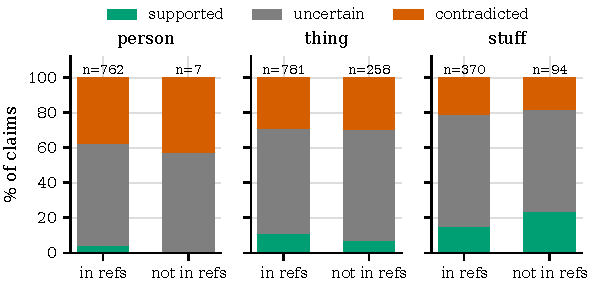
\includegraphics[width=\columnwidth]{figures/verdict_by_kind.pdf}
\caption{Verdicts of the attention-selected regions under the provisional thresholds, by claim kind and by whether a reference mentions the claimed class (raw attention).}
\label{fig:verdict}
\end{figure}

\subsection{Retell: Zero-Initialisation and First Training Runs}
\label{sec:exp-gate}
\textbf{Zero-initialisation.} Before the first update, every trained system reproduced the B0 draft exactly on the 200 validation images checked (\InitIdentical{} systems identical, beam search, same decoding settings). This holds by construction ($\tanh(0)=0$), but the check guards against implementation errors in the wrapped decoder. The pathway has \ParamsM\,M trainable parameters.

\textbf{First runs.} Table~\ref{tab:retell} reports one training run per system: three epochs on the half-B drafts with corruption rate $\rho=0.15$, evaluated on validation. These runs test that the full pipeline trains end to end and show how much the evidence moves the output. They are not tests of H1--H5, which need human labels and calibrated thresholds. These first runs used the earlier region rules and provisional thresholds. They establish an implementation baseline; they do not measure Retell performance with the frozen Look v2 records. Retell must be reassessed after Check calibration.

\begin{table*}[t]
\caption{Retell development runs on the validation split (decoder fine-tuned on A, pathway trained on B, 3 epochs,
$\rho=0.15$ unless stated). Each round has its own matched no-evidence control B0+. BLEU-4 and CIDEr use our
simplified tokeniser (compare only with scores using the same tokenisation). \emph{Changed}: captions that
differ from the draft. \emph{Alt.\ adopt.} / \emph{Con.\ kept}: of the draft claims whose record is
\emph{contradicted}, the share whose alternative label appears in the output / whose claimed label is still in
the output (the set of contradicted records depends on the thresholds, so these two columns are comparable only
within a round). \emph{Sens.}: captions that change when all evidence is masked. All columns are automatic;
none is a human-verified error rate.}
\label{tab:retell}
\centering\footnotesize
\begin{tabular}{@{}lccccccc@{}}
\toprule
System & BLEU-4 & CIDEr & RUOR & Changed (\%) & Alt.\ adopt.\ (\%) & Con.\ kept (\%) & Sens.\ (\%) \\
\midrule
B0 (draft) & 32.6 & 0.979 & 15.8 & -- & -- & -- & -- \\
B1 (word repl., provisional thr.) & 27.9 & 0.815 & 25.9 & 40.3 & -- & -- & -- \\
\midrule
\multicolumn{8}{@{}l}{\emph{Round 1: provisional thresholds, no patch dropout}} \\
B0+ (no evidence) & 34.0 & 0.983 & 15.7 & 63.6 & -- & -- & -- \\
LCR, raw attention & 34.2 & 0.987 & 15.8 & 65.0 & 15.1 & 90.3 & -- \\
LCR, sink-corr. attention & 34.3 & 0.991 & 15.7 & 64.1 & 41.0 & 87.1 & 10.9 \\
B3 (detector regions) & 34.1 & 0.981 & 15.8 & 64.6 & 26.5 & 88.8 & -- \\
B2 (image tags) & 34.3 & 0.983 & 15.7 & 64.7 & -- & -- & -- \\
\bottomrule
\end{tabular}
\end{table*}

\begin{table}[t]
\caption{Evidence interventions on validation: the same trained model with real records, all records masked
(null token only), or false records (alternative label of each contradicted record replaced by a class the
detector does not see in the image). \emph{Sens.}: captions that differ from the real-evidence output.
[R1]/[R2]: development round.}
\label{tab:interv}
\centering\footnotesize\setlength{\tabcolsep}{3pt}
\begin{tabular}{@{}p{2.3cm}lcccc@{}}
\toprule
System & Evidence & CIDEr & RUOR & Alt.\ adopt. & Sens.\ (\%) \\
\midrule
LCR, raw attention [R1] & real & 0.987 & 15.8 & 15.1 & -- \\
 & masked & 0.993 & 15.8 & 15.2 & -- \\
 & false & 0.987 & 15.8 & 0.0 & -- \\
\addlinespace
LCR, sink-corr. attention [R1] & real & 0.991 & 15.7 & 41.0 & -- \\
 & masked & 0.984 & 15.9 & 41.0 & 10.9 \\
 & false & 0.991 & 15.7 & 0.0 & 0.0 \\
\addlinespace
B3 (detector regions) [R1] & real & 0.981 & 15.8 & 26.5 & -- \\
 & masked & 0.990 & 15.7 & 27.6 & -- \\
 & false & 0.981 & 15.8 & 0.0 & -- \\
\bottomrule
\end{tabular}
\end{table}


\begin{figure}[t]
\centering
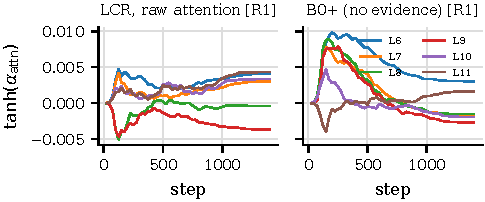
\includegraphics[width=\columnwidth]{figures/gate_curves.pdf}
\caption{Attention-gate values $\tanh(\alpha_{\text{attn}})$ of the six gated blocks during training, for LCR and for the no-evidence control B0+.}
\label{fig:gates}
\end{figure}

\subsection{Annotation Tool and Error Pilot}
The blinded annotation page (Section~\ref{sec:design-eval}) has been generated for the 100-image error pilot. It contains the B0 drafts of 100 randomly drawn validation images and asks for a label for every concrete noun, including nouns outside $V$. Labelling by two team members is the next step. Their labels will give the first human estimate of the draft error rate, Cohen's $\kappa$, and the data needed to set the verdict thresholds and fix the test sample size (Table~\ref{tab:power}).
